\section{\ref{rq:finding-changes} How can we find changes between two models?}

\todo{This section must have an introduction}

Finding changes is handled in the \verb|Testar.ChangeDetection.Core.Algorithm| namespace. The algorithm can be used by different project, for example by an application for CI integration. The visualisation of the differences are handled by the new analysis website and are discussed in section \ref{rq:type-visualisation-answer}. The classes used for the algorithm are visualised in figure \ref{fig:class-diagram-differences}. 

\begingroup
\captionsetup{type=figure}
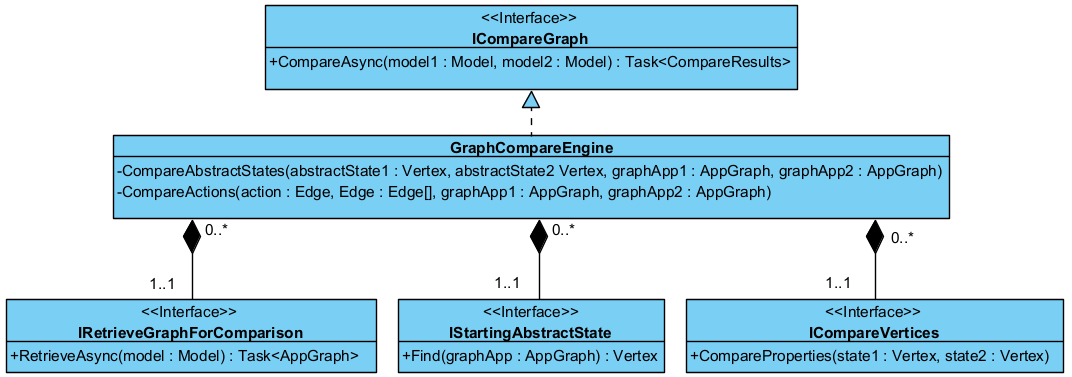
\includegraphics[scale=0.65]{images/4-UML-Differences.png}
\captionof{figure}{Class diagram, algorithm namespace (UML 2.0)}\label{fig:class-diagram-differences}
\endgroup

\subsection{The change detection algorithm} \label{sec:change-detection-algorithm}
In this sub section the algorithm will be explained stating with a high level overview. After the high level overview the different interfaces in figure \ref{fig:class-diagram-differences} are explained in more detail.

The concept of \textit{corresponding states} need to be explained to understand the algorithm. Corresponding states means that there are two states, in the new and in the old model, that are identify as the 'same' state but can have different data. There are a couple of ways to identify corresponding states. The first is by assumption, the second is inferred and the last is by asking a third party (for example a human input). For the developed algorithm only the first two are used. 

Figure \ref{fig:compare-algorithm-start} gives an overview of the start of the algorithm. The \verb|GraphCompareEngine| starts with retrieving the graph data for the old and the new model. This is indicated by step 1.1, step 1.2 follows identical steps as 1.1 and is omitted from the diagram.
\newpage

\begingroup
\captionsetup{type=figure}
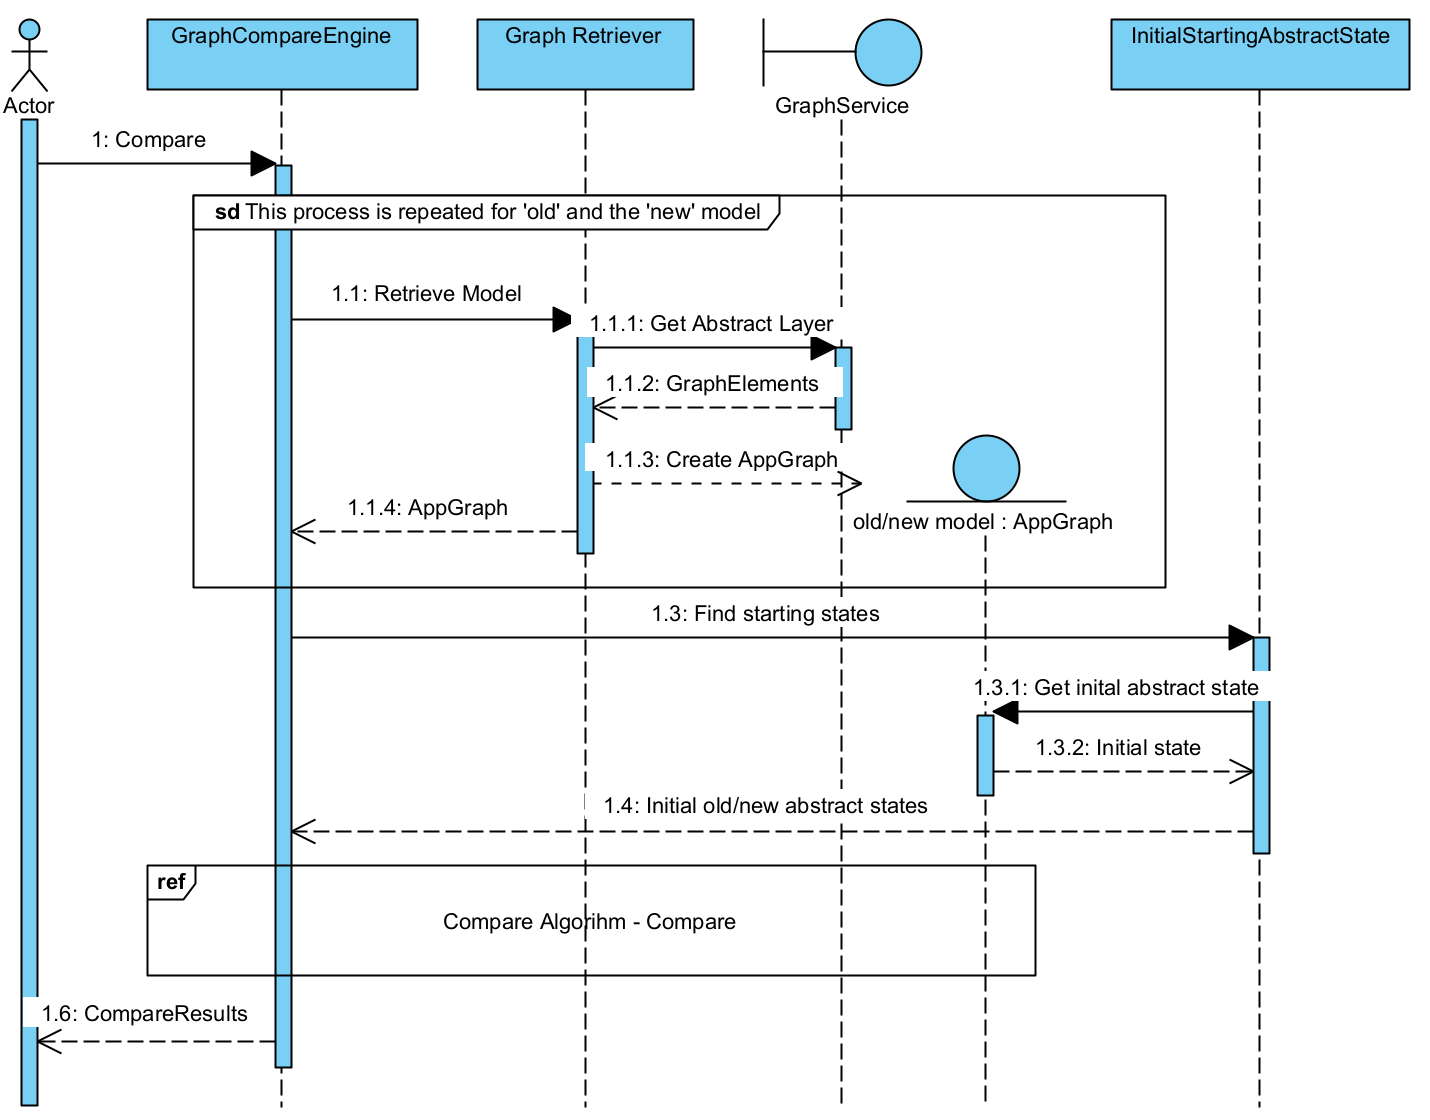
\includegraphics[scale=0.9]{content/5-Results/Images/Compare-algorithm-start.png}
\captionof{figure}{Compare Algorithm (1) - Start (UML 2.0)}\label{fig:compare-algorithm-start}
\endgroup

The next step is finding the starting states, indicated by step 1.3. Those will be the first corresponding states. The current version of the algorithm assumes that the initial states from both graph are corresponding. Those states could, for example, be a splash screen or a loading screen.

The flow of the algorithm continues in figure \ref{fig:compare-algorithm-compare} with 1.5. in which the initial states are marked as corresponding states (Step 1.5.1). The rest of the progress follows a recursive pattern between two methods of the algorithm, the first \verb|CompareAbstractStates| (Step 1.5) and \verb|CompareActions| (Step 1.5.5).

The algorithm is using the abstract model to find high level changed within the system under tests. As discussed in section \ref{abstract-model} the concrete model contains all the information about states within the application under test, the abstract model contains the abstracted data. Concrete states are abstracted in abstract states and concrete actions are abstracted into abstract actions. As so the a abstract state contains one or more abstract actions, leading to another abstract state. 
In the step 1.5 the corresponding states are compared. The first step is settings the \verb|IsHandeld| variable to make sure states are not compared twice. Then the element data of the two abstract states is compared. This is done by the \verb|ICompareVertices| interface and is discussed in more detail on the sub subsection on page \pageref{sec:i-compare-vertices}.

The last step of the \verb|CompareAbstractStates| step is enumerating over the abstract actions of the new model. For each action the method \verb|CompareActions| (step 1.5.5) is executed which also marks the action of the new model as handled. Then it looks in the corresponding abstract state for an action with the same \verb|actionId|. The action id is a hashed subset of properties and was discussed in section \ref{state-identifiers}. 

If an abstract action is found with the same \verb|actionId|, it then retrieves the target state of both actions. When both states are not handled it will call the \verb|CompareAbstractStates| (Step 1.5) to make the recursive call. Both states are marked as corresponding states. This is the second approach of finding corresponding states; inferring the corresponding states by walking through the two graphs. 

The code for the change detection algorithm is handheld by four interface. Each interface is discussed in more detail below starting with the \verb|IRetrieveGraphForComparison| interface which downloads the graph for comparison. Secondly the \verb|IStartingAbstractState|, responsible for finding the staring states for the comparison, then the \verb|ICompareVertices| interface, which compares the element data for two given vertexes. The last interface is \verb|ICompareGraph| which will execute the algorithm and has a dependency on the discussed the interfaces. 

In the coming sections, the various interface and associated default implementations are explained in more detail.

\textit{Note: When comparing the methods and return values of the presented in this thesis and the source code one can find a discrepancy. Some are return values are decorated with the} \verb|Task<..>| \textit{object and some method have the suffix} \verb|Async|. \textit{Those technical details are omitted from the thesis since they do not provide any additional value to the algorithm. When a method return in C\# it is an asynchronous method that can be awaited by the called. The} \verb|await| \textit{keyword will create a non-blocking call that enabled multi threading applications \cite{asynchronous-programming}.}

\newpage


\begingroup
\captionsetup{type=figure}
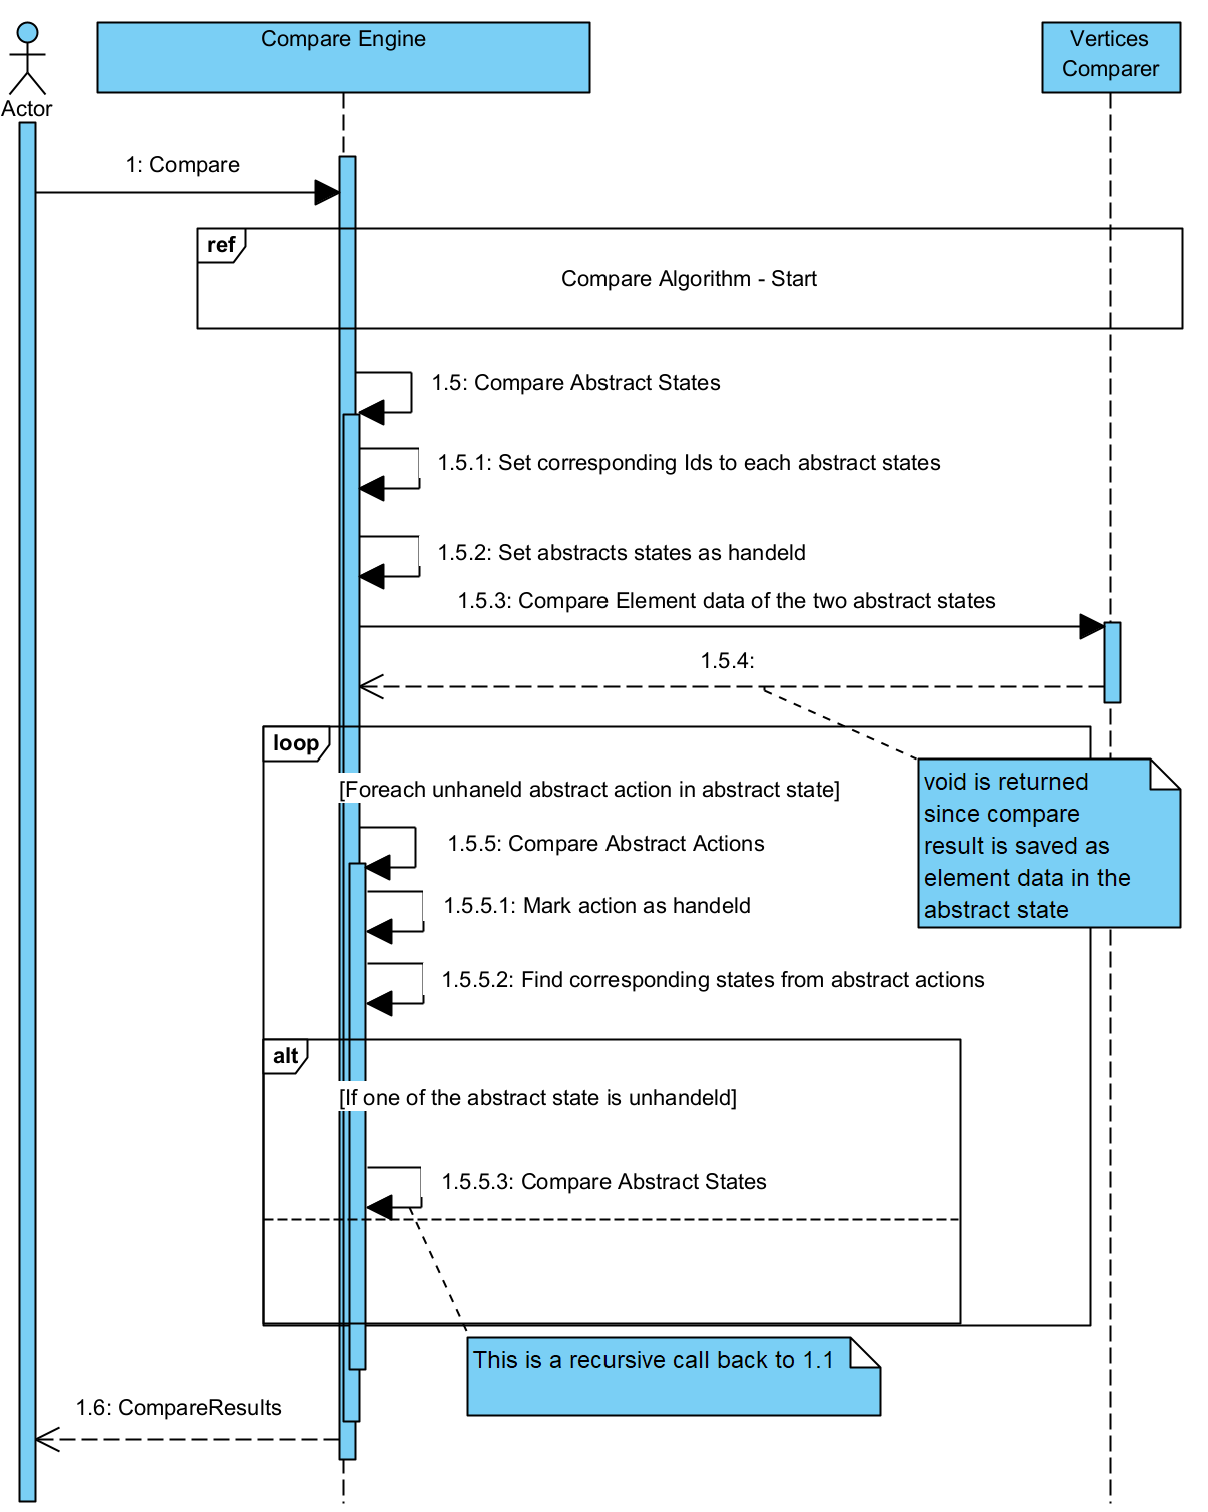
\includegraphics[scale=0.9]{content/5-Results/Images/Compare-algorithm-compare.png}
\captionof{figure}{Compare Algorithm (2) - Compare (UML 2.0)}\label{fig:compare-algorithm-compare}
\endgroup

\subsubsection{IRetrieveGraphForComparison}
The \verb|IRetrieveGraphForComparison| interface is implemented by the \verb|GraphForCompareRetriever|, and is responsible for retrieving the graph data from the server. It has a dependency on the GraphService (\ref{sec:the-graph-service}). 

Given a \verb|Model|, which contains the application name and version, the data from the abstract Layer, the concrete Layer and the abstract concrete connectors are retrieved. Only the data from the abstract layer is used for the comparison. The data from the concrete layer and the abstract concrete connectors are downloaded so that they can be used in the visualisation of the presentation of the graph (Discussed in more detail in \ref{rq:type-visualisation-answer}), likewise is the enrichment of the abstract actions with the description from the corresponding concrete actions.

\begingroup
\captionsetup{type=figure}
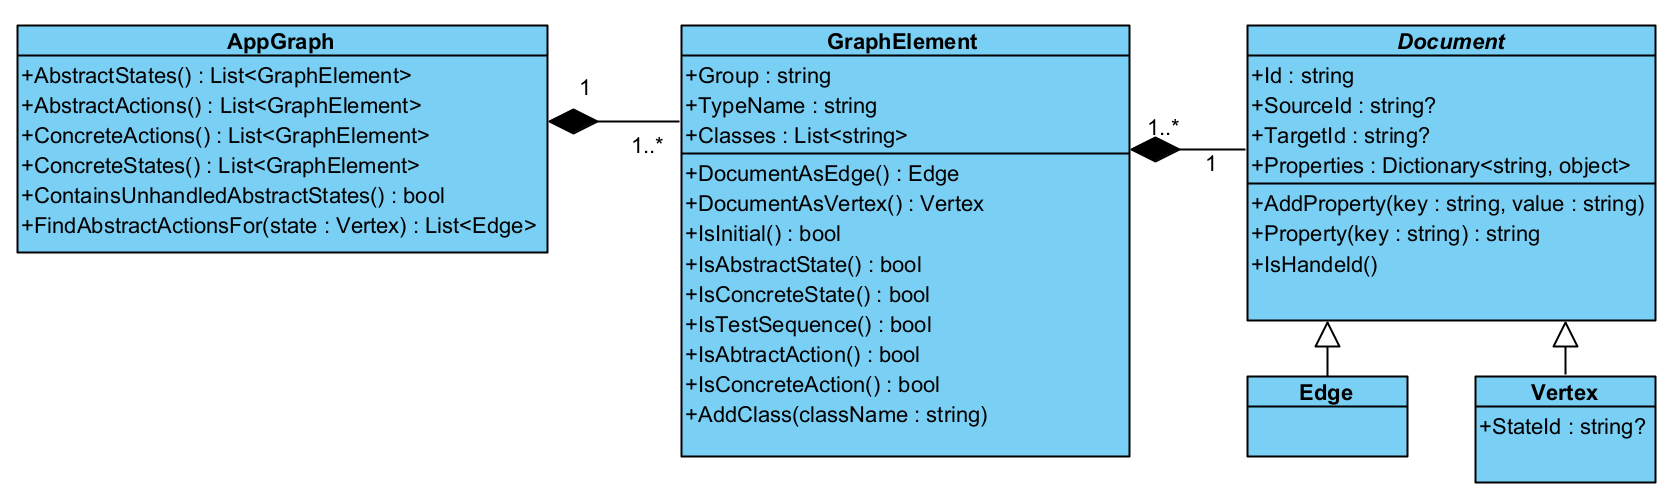
\includegraphics[scale=0.6]{images/4-UML-Models.png}
\captionof{figure}{Class diagram Graph models (UML 2.0)}\label{fig:class-diagram-models}
\endgroup

The \verb|AppGraph| class, shown in figure \ref{fig:class-diagram-models}, is wrapper around a collection of \verb|GraphElement|'s. The \verb|GraphElement| is container a abstract Document which is either a Vertex or an Edge. The abstract \verb|Document| class contains the properties from the vertex or the Edge.

%When the \verb|AppGraph| is serialised into JSON, it will generated the structure that can be read by the Cytoscape Graph visualisation library.

Although the data for each element is located as set of properties, the classes in figure \ref{fig:class-diagram-models} contains some helper properties, e.g. \verb|IsAbstractAction| and \verb|IsConcreteState| which returns a Boolean depending on the type name. 

\subsubsection{IStartingAbstractState} \label{sec:starting-abstract-state}
The interface \verb|IStartingAbstractState| is used to locate at which abstract state the algorithm must start comparing. The default implementation is given by the \verb|InitialStartingAbstractState|. As the name of the class suggest this implementation is looking for the initial state. For a correct working of the algorithm it is assumed that the initial states are corresponding states. This can be a splash or a loading screen for example.

\subsubsection{ICompareVertices} \label{sec:i-compare-vertices}
When the algorithm finds corresponding states it needs to compare the states together. This comparison is handled by the \verb|ICompareVertices| interface. A default implementation is provided by the \verb|CompareVertices| class. In algorithm \ref{alg:comparison-corresponding-states} is explained how the inner workings of the implementation is working.  

\begin{algorithm}
    \caption{Vertex comparison}\label{alg:comparison-corresponding-states}
    \begin{algorithmic}
        \Require Element data of old model
        \Require Element data of new model
        \State $O$ = Element data of old model
        \State $N$ = Element data of new model
        \For{$p \in$ $(O \cup N)$}
            \State Mark $p$ as \textit{Added} in new model
        \EndFor
        \For{$p \in$ $(N \cup O)$}
            \State Mark $p$ as \textit{Removed} in old model
        \EndFor
        \For{$p \in$ $(O \cap N)$}
            \State $Ov$ = value of element data in old model
            \State $Nv$ = value of element data in new model
            \If{$Ov \neq Nv$}
               \State Mark element data as changed 
            \EndIf
        \EndFor
    \end{algorithmic}
\end{algorithm}

All the finding of algorithm \ref{alg:comparison-corresponding-states} are saved as element data with the prefix \verb|CD_| (for Change Detection) so that the visualisation can find them easy. Moreover, changed element data is prefixed with \verb|CD_CO_| or \verb|CD_CN_| (respectively CO standing for Changed Old value and CN for Changed New value), new data elements are prefixed with \verb|CD_A_| (A for added) and removed data elements are prefixed with \verb|CD_R_| (R for removed).

\subsubsection{ICompareGraph} \label{sec:compare-algorithm}
At the start of this section (\ref{sec:change-detection-algorithm}) an high level overview is given concerning the change detection algorithm. The algorithm is implemented by in the \verb|GraphCompareEngine| class and is using the above mentioned inteffaces as dependencies. The \verb|Compare| method is given 

A limitation of change detection is that the object, in this case the old and new version of an application, needs to be similar enough to enable the detection of changes in the first place \cite{andrews2009visual}. To verify this requirement, the used abstract attributes of the two versions are compared and when different abstract attributes are used, the comparison process is canceled \cite{stateDiff}. 

%Abstract Graph comparison
%First the software create a ComparableGraph. A Comparable graph only contacts the nodes and edges from the abstract states and abstract actions. The data however will include data from the concrete states and actions. 

%When we have a changed abstractstate, get a widgettree of one concrete state
%https://www.xmlunit.org/  have a package for both java as .NET to create differences between version.

%using a fast mode
%the fast mode will only look into changes on the abstract level. Changes like different colours for example


% Every element has an ID generated by OrientDb e.g. #154:0. When merging elements those Id's are merged to by the following algorithm: \#Id1\_Id2 e.g. \#150:0\_\#150:1. 

%difference engine
%merge graph \cite{andrews2009visual}
%the graph needs to be similar are "enough"

%Finding matching notes is done by the difference algorithm. 

